\documentclass[main.tex]{subfiles}
\begin{document}

\section{Introduction}

\subsection{Preliminaries}

We will have convention that for a space time vector $x$ in a chosen frame of reference $\bs{x}$ will mean space part of the vector $x$. $x\cdot y$ will mean Minkowsky inner product:
\begin{equation}
x\cdot y = x^0 y^0 - \bs{x}\cdot \bs{y},
\end{equation}

where $\bs{x}\cdot \bs{y}$ is euclidean inner product in $\R^3$. We will also write $x^2 = x\cdot x$ and $\bs{x}^2 = \bs{x}\cdot\bs{x}.$

When a particle of mass $m$ has a $4$-momentum $p$, 
we will denote it's energy by $E_{\bs{p}} = p^0$. 
Note that

\begin{equation}
E_{\bs{p}} = \sqrt{\bs{p}^2 + m^2}.
\end{equation}

\begin{fact}
If $p, q$ are $4$-momentums of particles of mass $m$, then the expression
\begin{equation}
E_{\bs{q}}\delta^{(3)}(\bs{p} - \bs{q})
\end{equation}
is Lorentz invariant. 
\end{fact}
\begin{proof}
Take Lorentz transformation
\begin{equation}
\begin{cases}
E_{\bs{p}'} = p'^0 = \gamma p^0 - \beta\gamma p^1, \\
p'^1 = \gamma p^1 - \beta\gamma E_{\bs{p}}.
\end{cases}
\end{equation}

Let's calculate 
\begin{multline*}
\\
\delta^{(3)}(\bs{p'} - \bs{q'}) = \delta((p'^1 - q'^1, p'^2 - q'^2, p'^3 - q'^3))\\
= \delta((\gamma p^1 - \beta\gamma E_{\bs{p}} - \gamma q^1 + \beta\gamma E_{\bs{q}},p^2 - q^2, p^3 - q^3)).\\
\\
\end{multline*}
Note that
\begin{equation}
\cfrac{\partial}{\partial p^k} E_{\bs{p}} = \cfrac{\partial}{\partial p^k} \sqrt{\bs{p}^2 + m^2} =
\cfrac{p^k}{E_{\bs{p}}}.
\end{equation}

Then 
\begin{multline*}
\\
\cfrac{\partial}{\partial p^1}(\gamma p^1 - \beta\gamma E_{\bs{p}} - \gamma q^1 + \beta\gamma E_{\bs{q}})\\
\\ = \gamma - \cfrac{\beta\gamma p^1}{E_{\bs{q}}} = \cfrac{E_{\bs{p}}\gamma - \beta\gamma p^1}{E_{\bs{p}}} = \cfrac{E_{\bs{p}'}}{E_{\bs{p}}}.
\\ 
\end{multline*}

Let's write Jacobian

\begin{equation}
\bigg|\cfrac{\partial(\bs{p'} - \bs{q'})}{\partial \bs{p}} \bigg|=
\begin{vmatrix}
\cfrac{E_{\bs{p}'}}{E_{\bs{p}}} & \cfrac{\beta\gamma p^2}{E_{\bs{p}}} & \cfrac{\beta\gamma p^3} 
{E_{\bs{p}}} \\
0 & 1 & 0 \\
0 & 0 & 1
\end{vmatrix} = \cfrac{E_{\bs{p}'}}{E_{\bs{p}}}.
\end{equation}

By Theorem \ref{delta-zeros}, we have
\begin{equation}
 \delta(\bs{p}' - \bs{q}') = \bigg(\bigg|\cfrac{\partial(\bs{p'} - \bs{q'})}{\partial \bs{p}} \bigg|_{\bs{p}=\bs{q}}\bigg)^{-1} \delta(\bs{p} - \bs{q}) =
\cfrac{E_{\bs{q}}}{E_{\bs{q}'}} \delta(\bs{p} - \bs{q}).
\end{equation}




Thus
\begin{equation}
E_{\bs{q}'} \delta^{(3)}(\bs{p'} - \bs{q'}) = E_{\bs{q}}\delta^{(3)}(\bs{p} - \bs{q}).
\end{equation}
\end{proof}

\paragraph{Klein-Gordon equation}

For a relativistic particle $E^2 = \bs{p}^2 + m^2$, there is an idea for relativistic  Schrödinger equation
\begin{equation}
i\hbar \cfrac{\partial}{\partial t}\ket{\phi(t)} =  \sqrt{\bs{P}^2 + m^2} \ket{\phi(t)}.
\end{equation}

which is a motivation for a "squared" version (we will set $\hbar=1$):
\begin{equation}
-\cfrac{\partial^2}{\partial t^2} = \bs{P}^2 + m^2,
\end{equation}
which is
\begin{equation}
-\cfrac{\partial^2}{\partial t^2} = -\nabla^2 + m^2,
\end{equation}
or
\begin{equation}
\cfrac{\partial^2}{\partial t^2} - \nabla^2 + m^2 = 0.
\end{equation} 
Can be noted using raised index of partial derivative and Einstein summation convention:
\begin{equation}
\partial^\mu\partial_\mu + m^2 = 0.
\end{equation}
From this immediately follows Lorentz invariance, but we will give a direct proof in language of tensor transformations Figure \ref{klein-proof}.

\begin{figure}[H]
\label{klein-proof}
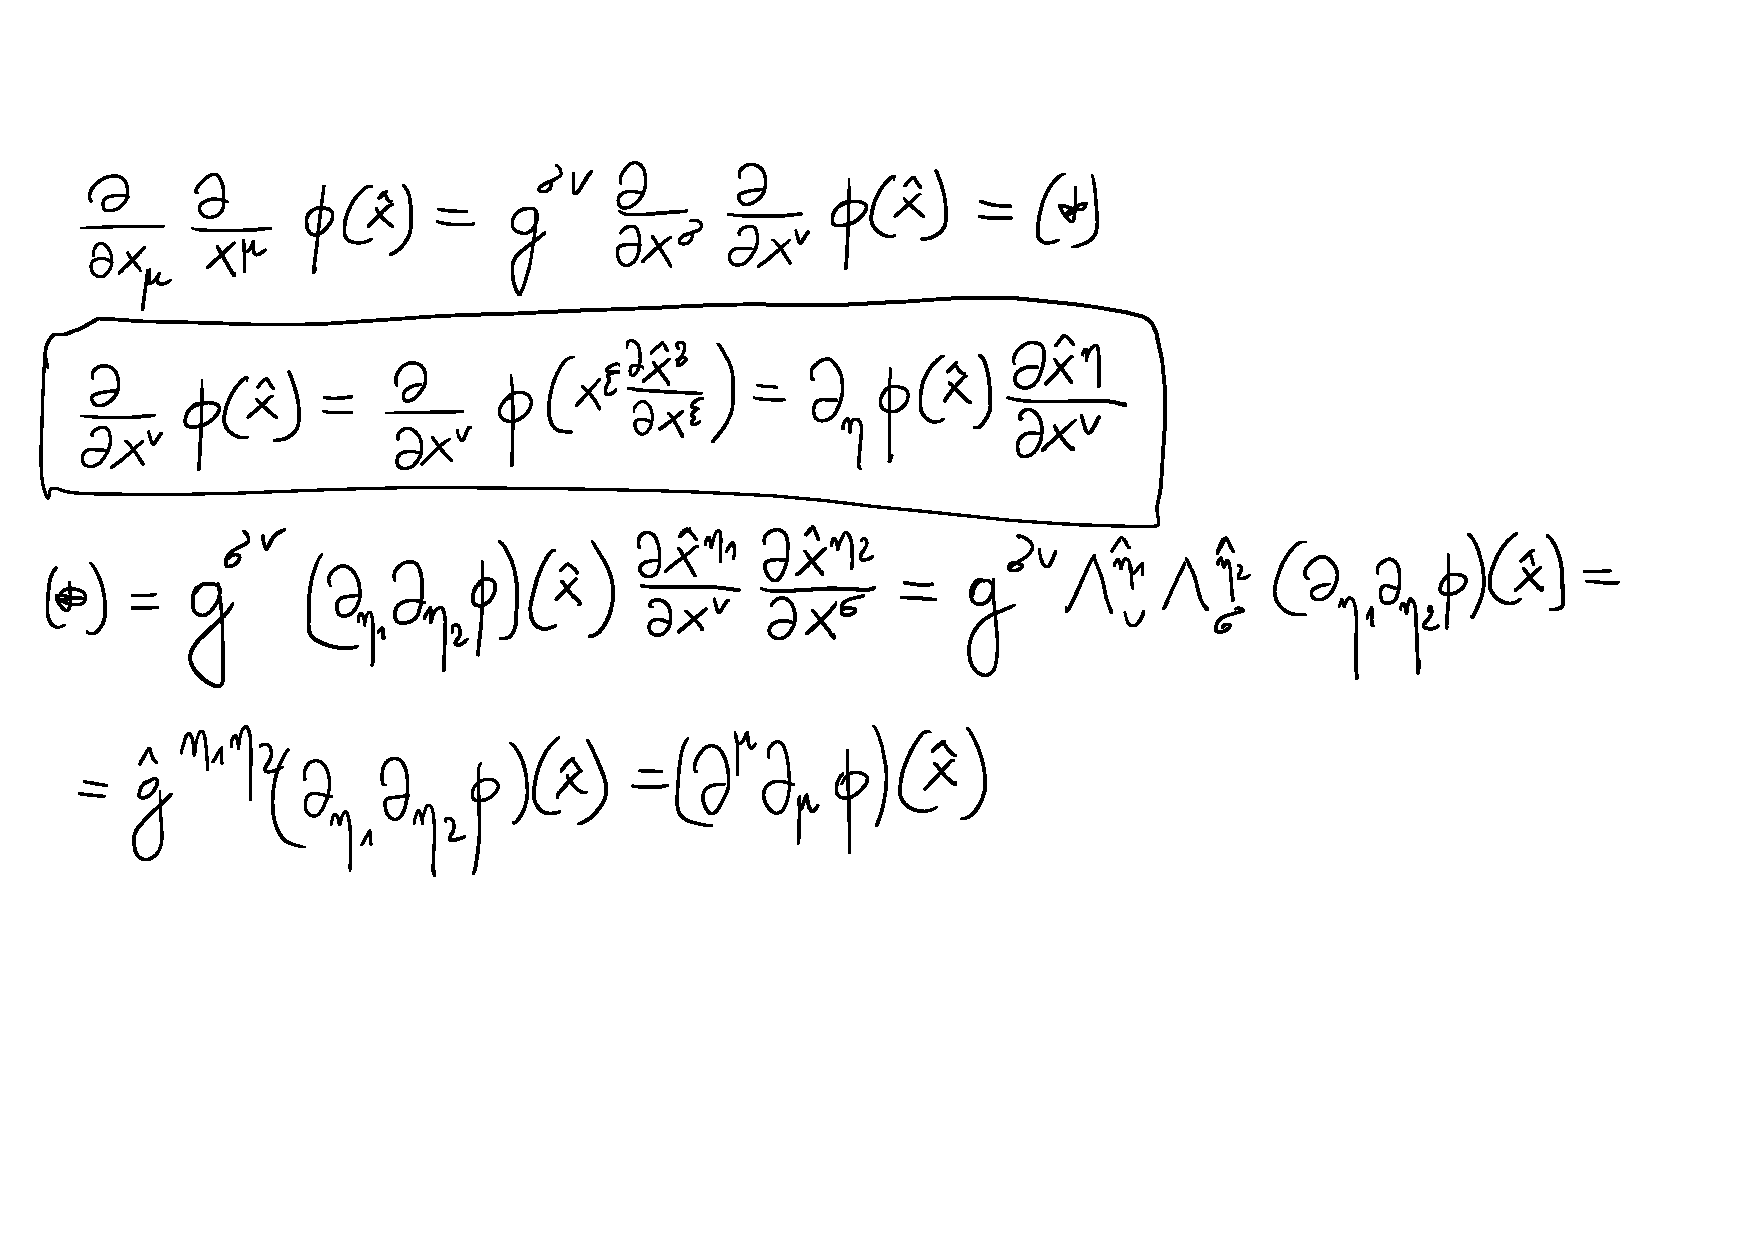
\includegraphics[scale=0.5]{figs/KleinInvariance}
\caption{Proof of Lorentz invariance of Klein-Gordon equation}
\end{figure}
\subsection{Creation and anihilation algebra for bozons and fermions}
In this subsection $p$ indexes are arbitrary and they are not necesarlily related to momentum. 

We are still in a ``usual" Dirac formulation of quantum mechanics. We simply make certain assumptions about family of operators $a_p$ and one distinguished state    $\ket{0} \not= 0$, which is called a vaccume state.

\begin{definition}[Bozonic creation and anihilation assumptions]
We will call the bellow statements \textit{bozonic creation and anihilation assumptions}
\begin{align}
& [a_p, a^\dagger_q] = \delta(p - q),\\
& [a_p, a_q] = 0 \text{ and } [a^\dagger_p, a^\dagger_q] = 0,\\
& a_p\ket{0} = 0.
\end{align}
\end{definition}

\begin{proposition}
Under bozonic creation and anihilation assumptions, we have
\begin{equation}
\label{anihilation-operator-characteristic}
a_p (a_{q_1}^\dagger \dots a_{q_n}^\dagger) = \sum_{k=1}^n\delta(p - q_k) a_{q_1}^\dagger a_{q_{k - 1}}^\dagger \dots a_{q_{k + 1}}^\dagger a_{q_n}^\dagger + (a_{q_1}^\dagger \dots a_{q_n}^\dagger)a_p.
\end{equation}
\end{proposition}
\begin{proof}
Note that (\ref{anihilation-operator-characteristic}) holds for $n = 1$. We will prove it by induction. Let's now assume (\ref{anihilation-operator-characteristic}) holds for $n - 1$.
\begin{align*}
& a_p (a_{q_1}^\dagger \dots a_{q_n}^\dagger)=
a_{q_1}^\dagger a_p (a_{q_2}^\dagger \dots a_{q_n}^\dagger) + \delta(p - q_1) (a_{q_2}^\dagger \dots a_{q_n}^\dagger)= \\
& a_{q_1}^\dagger\sum_{k=2}^n\delta(p - q_k) a_{q_2}^\dagger a_{q_{k - 1}}^\dagger \dots a_{q_{k + 1}}^\dagger a_{q_n}^\dagger + \delta(p - q_1) (a_{q_2}^\dagger \dots a_{q_n}^\dagger) + a_{q_1}^\dagger (a_{q_2}^\dagger \dots a_{q_n}^\dagger)a_p.
\end{align*} 
\end{proof}

\begin{corollary}
\begin{equation}
a_p (a_{q_1}^\dagger \dots a_{q_n}^\dagger) \ket{0} = \sum_{k=1}^n\delta(p - q_k) a_{q_1}^\dagger a_{q_{k - 1}}^\dagger \dots a_{q_{k + 1}}^\dagger a_{q_n}^\dagger \ket{0}.
\end{equation}
\end{corollary}

\begin{corollary}
\begin{equation}
a_p (a_{q}^\dagger)^n \ket{0} = n \delta(p - q) (a_{q}^\dagger)^{n-1} \ket{0}.
\end{equation}
\end{corollary}

\begin{lemma}
If $[a_p, a^\dagger_q] = \delta(p - q)$, then
\begin{align*}
&\int K_1(\dots, p, q, \dots) a_p a^\dagger_q K_2(\dots, p, q, \dots) d \dots dpdq \ldots = \\
&\int K_1(\dots, p, q, \dots) a^\dagger_q a_p K_2(\dots, p, q, \dots) d \dots dpdq \ldots + \\ 
&\int K_1(\dots, p, p, \dots)K_2(\dots, p,p, \dots)d \dots dp \dots.
\end{align*}
\end{lemma}

\begin{proposition} We assume bozonic creation and anihilation assumptions.
Let $F = \int dp\, f(p)a^\dagger_p a_p$ and $G = \int dp\, g(p)a^\dagger_p a_p$, then
\begin{equation}
[F, G] = 0.
\end{equation} 
\end{proposition}
\begin{proof}
\begin{align*}
&FG = \int dp dq \,f(p)g(q) a^\dagger_p a_p a^\dagger_q a_q = \\
& \int dp dq f(p)g(q) a^\dagger_p  a^\dagger_q a_p a_q + \int dp f(p)g(p) a^\dagger_p a_p =  \\
& \int dp dq f(p)g(q) a^\dagger_q a^\dagger_p  a_q  a_p  + \int dp f(p)g(p) a^\dagger_p a_p \\ =
& \int dp dq f(p)g(q) a^\dagger_q a_q a^\dagger_p   a_p - \cancel{\int dq f(q)g(q) a^\dagger_q    a_q}  + \cancel{\int dp f(p)g(p) a^\dagger_p a_p} 
= GF. \\ 
\end{align*}
\end{proof}

\begin{proposition}
We assume bozonic creation and anihilation assumptions. Let $P = \int pdp\, a^\dagger_p a_p$ and
\begin{equation}
\hat{V} = \int dp_1 dp_2 dq\, V_q a^\dagger_{p_1 + q} a^\dagger_{p_2 - q} a_{p_2}a_{p_1}, 
\end{equation}
then $[\hat{V}, P] = 0.$
\end{proposition}
\begin{proof}
Let's do calculations:
\begin{figure}[H]
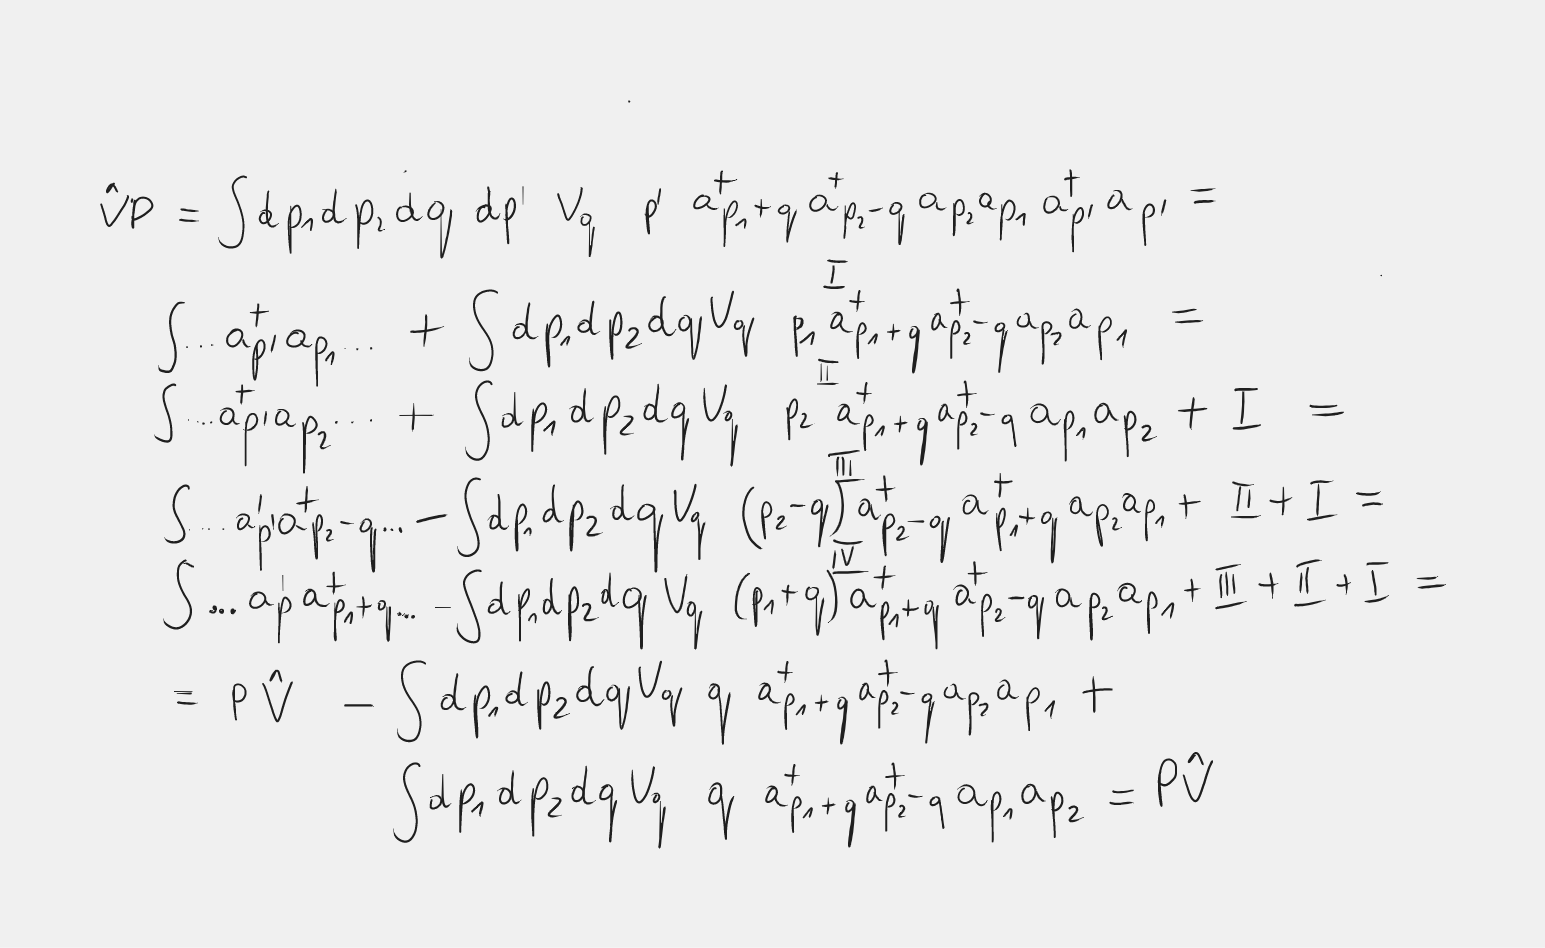
\includegraphics[width=\textwidth]{figs/two_body_potential}
\end{figure}

\end{proof}

Let's now work out a more generic equations which will work with bozons as well as with fermions. For that it will be usefull to introduce a generic commutator expression
\begin{equation}
[A, B]_{\zeta} \stackrel{def}{=} AB -\zeta BA.
\end{equation}

Note that for commutator, we have $[A, B] = [A, B]_1$ and for anticommutator, we have $\{A, B\} = [A, B]_{-1}$.

Note a usefull transposition:
\begin{equation}
AB = [A, B]_{\zeta} + \zeta BA.
\end{equation}

\begin{assumption}
\label{anihilation-creation-assumptions}
Let $\zeta\in\{-1, 1\}$. Assume that the bellow conditions holds for a family of operators $a_p$.
\begin{align}
& [a_p, a^\dagger_q]_\zeta = \delta(p - q),\\
& [a_p, a_q]_\zeta = 0 \text{ and } [a^\dagger_p, a^\dagger_q]_\zeta = 0,\\
& a_p\ket{0} = 0.
\end{align}
\end{assumption}

For $\zeta = 1$ the above are \textit{bozonic anihilation and creation assumptions}, for $\zeta = -1$ the above are \textit{fermionic anihilation and creation assumptions}.

Note that under Assumption \ref{anihilation-creation-assumptions}, we have always

\begin{equation}
a_p a_{q}^\dagger = \delta(p - q) + \zeta a_{q}^\dagger a_p,
\end{equation}

\begin{equation}
a_{q}^\dagger a_p = \zeta \delta(p - q) - \zeta a_p a_{q}^\dagger,
\end{equation}

\begin{equation}
a_p a_q = \zeta a_q a_p,
\end{equation}

\begin{equation}
a^\dagger_p a^\dagger_q = \zeta a^\dagger_q a^\dagger_p.
\end{equation}  

Note that it follows that for fermions we have $a^\dagger_p a^\dagger_p = 0$. For all subsequent calculations it is also worth to remeber that $\zeta^{2k} = 1$ for any integer $k$.

\begin{proposition}
Under Assumption \ref{anihilation-creation-assumptions}, we have
\begin{equation}
\label{anihilation-operator-characteristic}
a_p (a_{q_1}^\dagger \dots a_{q_n}^\dagger) = \sum_{k=1}^n \zeta^{k - 1} \delta(p - q_k) a_{q_1}^\dagger \dots a_{q_{k - 1}}^\dagger a_{q_{k + 1}}^\dagger  \dots  a_{q_n}^\dagger + \zeta^n( a_{q_1}^\dagger \dots a_{q_n}^\dagger)a_p.
\end{equation}
\end{proposition}
\begin{proof}
Note that (\ref{anihilation-operator-characteristic}) holds for $n = 1$. We will prove it by induction. Let's now assume (\ref{anihilation-operator-characteristic}) holds for $n - 1$.
\begin{align*}
& a_p (a_{q_1}^\dagger \dots a_{q_n}^\dagger)=
\zeta a_{q_1}^\dagger a_p (a_{q_2}^\dagger \dots a_{q_n}^\dagger) + \delta(p - q_1) (a_{q_2}^\dagger \dots a_{q_n}^\dagger)= \\
& \zeta a_{q_1}^\dagger\sum_{k=2}^n\zeta^k \delta(p - q_k) a_{q_2}^\dagger \dots a_{q_{k - 1}}^\dagger a_{q_{k + 1}}^\dagger  \dots a_{q_n}^\dagger + \zeta^0 \delta(p - q_1) (a_{q_2}^\dagger \dots a_{q_n}^\dagger) \\
& + \zeta a_{q_1}^\dagger \zeta^{n - 1}(a_{q_2}^\dagger \dots a_{q_n}^\dagger)a_p = \\
& \sum_{k=1}^n \zeta^{k - 1} \delta(p - q_k) a_{q_1}^\dagger a_{q_{k - 1}}^\dagger \dots a_{q_{k + 1}}^\dagger a_{q_n}^\dagger + \zeta^n( a_{q_1}^\dagger \dots a_{q_n}^\dagger)a_p.
\end{align*} 
\end{proof}

\begin{corollary}
Under Assumption \ref{anihilation-creation-assumptions}, we have
\begin{equation}
a_p (a_{q_1}^\dagger \dots a_{q_n}^\dagger) \ket{0} = \sum_{k=1}^n\zeta^{k-1} \delta(p - q_k) a_{q_1}^\dagger \dots a_{q_{k - 1}}^\dagger a_{q_{k + 1}}^\dagger  \dots a_{q_n}^\dagger \ket{0}.
\end{equation}
\end{corollary}

\begin{proposition}
\label{count-operators}
Under Assumption \ref{anihilation-creation-assumptions} for $F = \int dp\, f(p)a^\dagger_p a_p$, we have
\begin{equation}
F a^\dagger_{p_1} \dots a^\dagger_{p_n}\ket{0} = \bigg( \sum_{k = 1}^n f(p_k)\bigg) a^\dagger_{p_1}  \dots a^\dagger_{p_n}\ket{0}.
\end{equation}
\end{proposition}
\begin{proof}
\begin{align*}
& F a^\dagger_{p_1} \dots a^\dagger_{p_n}\ket{0} = \int dp\, f(p)a^\dagger_p a_p a^\dagger_{p_1}  \dots a^\dagger_{p_n}\ket{0} = \\
& \sum_{k=1}^n\zeta^{k-1} f(a_{p_k}) a^\dagger_{p_k}
a^\dagger_{p_1} \tdots \cancel{a^\dagger_{p_k}} \tdots a^\dagger_{p_n}\ket{0} = \\
& \sum_{k=1}^n\zeta^{k-1} \zeta^{k-1} f(a_{p_k}) a^\dagger_{p_1}  \dots a^\dagger_{p_n}\ket{0} = \\
& \bigg( \sum_{k = 1}^n f(p_k)\bigg) a^\dagger_{p_1}  \dots a^\dagger_{p_n}\ket{0}.
\end{align*}
\end{proof}

\begin{proposition} Under Assumption \ref{anihilation-creation-assumptions}, for
$F = \int dp\, f(p)a^\dagger_p a_p$ and $G = \int dp\, g(p)a^\dagger_p a_p$, we have
\begin{equation}
[F, G] = 0.
\end{equation} 
\end{proposition}
\begin{proof}
\begin{align*}
&FG = \int dp dq \,f(p)g(q) a^\dagger_p a_p a^\dagger_q a_q = \\
& \zeta \int dp dq \, f(p)g(q) a^\dagger_p  a^\dagger_q a_p a_q + \int dp\, f(p)g(p) a^\dagger_p a_p =  \\
& \zeta \int dp dq\, f(p)g(q) a^\dagger_q a^\dagger_p  a_q  a_p  + \int dp\, f(p)g(p) a^\dagger_p a_p \\ =
& \zeta \big( \zeta \int dp dq\, f(p)g(q) a^\dagger_q a_q a^\dagger_p   a_p - \zeta \int dq\, f(q)g(q) a^\dagger_q    a_q \big)  + \int dp\, f(p)g(p) a^\dagger_p a_p = \\
& \int dp dq\, f(p)g(q) a^\dagger_q a_q a^\dagger_p   a_p - \cancel{\int dq \, f(q)g(q) a^\dagger_q    a_q}  + \cancel{\int dp\, f(p)g(p) a^\dagger_p a_p} 
= GF. \\ 
\end{align*}
\end{proof}

We will know chnage $p, q$ notation to $\alpha, \beta$ (it is just notation change).

\begin{proposition}
Under Assumption \ref{anihilation-creation-assumptions}, for an operator defined as
\begin{equation}
V = \int d\alpha d\beta\, v(\alpha, \beta) a_{\alpha}^\dagger a_{\beta}^\dagger a_{\beta} a_{\alpha},
\end{equation}
we have
\begin{equation}
V a^\dagger_{\alpha_1} \dots a^\dagger_{\alpha_n}\ket{0} = \bigg(\sum_{k\not=k'}v(\alpha_k, \alpha_{k'})\bigg) a^\dagger_{\alpha_1} \dots a^\dagger_{\alpha_n}\ket{0}.
\end{equation}
\end{proposition}
\begin{proof}
\begin{align*}
& V a^\dagger_{\alpha_1} \dots a^\dagger_{\alpha_n}\ket{0} = \int d\alpha d\beta\, v(\alpha, \beta) a_{\alpha}^\dagger a_{\beta}^\dagger a_{\beta} a_{\alpha} a^\dagger_{\alpha_1} \dots a^\dagger_{\alpha_n}\ket{0} = \\
& \sum_{k = 1}^n \zeta^{k - 1} \int d\beta\, v(\alpha_k, \beta)a_{\alpha_k}^\dagger a_{\beta}^\dagger a_{\beta} (a^\dagger_{\alpha_1} \tdots \cancel{a^\dagger_{\alpha_k}} \tdots a^\dagger_{\alpha_n})\ket{0} = \\
& \sum_{k = 1}^n \zeta^{k - 1}\bigg( \sum_{k'=1}^{k - 1} \zeta^{k' - 1}  + \sum_{k'=k+1}^{n} \zeta^{k'}\bigg) v(\alpha_k, \alpha_{k'})a_{\alpha_k}^\dagger a_{\alpha_{k'}}^\dagger (a^\dagger_{\alpha_1} \tdots \cancel{a^\dagger_{\alpha_k}} \cancel{a^\dagger_{\alpha_{k'}}}\tdots a^\dagger_{\alpha_n})\ket{0} = \\
& \sum_{k = 1}^n \zeta^{k-1} \zeta^{k - 1}\bigg( \sum_{k'=1}^{k - 1} \zeta^{k'- 1}\zeta^{k' - 1}  + \sum_{k'=k+1}^{n} \zeta^{k'} \zeta^{k'}\bigg) v(\alpha_k, \alpha_{k'})
a^\dagger_{\alpha_1} \tdots a^\dagger_{\alpha_n}\ket{0} = \\
& \bigg(\sum_{k\not=k'}v(\alpha_k, \alpha_{k'})\bigg) a^\dagger_{\alpha_1} \dots a^\dagger_{\alpha_n}\ket{0}.
\end{align*}
\end{proof}

\subsection{Assembly of identical particles}

Assume we have a space of quantum states $\mathcal{X}$ which desribe single particle of a kind.

We will set $\zeta = 1$ (for bozons) or $\zeta = -1$ (for fermions). Let's define the following state:
\begin{equation}
\ket{\psi_1 \dots \psi_n} \stackrel{def}{=} \cfrac{1}{\sqrt{n!}}\sum_{\sigma\in S_n} \zeta^\sigma 
\ket{\psi_{\sigma(1)}} \dots \ket{\psi_{\sigma(n)}}. 
\end{equation}

The above should be understood with the convention that $1^\sigma = 1$ and $(-1)^\sigma$ is as defined in Definition \ref{permutation-sign}.

Note that this state belongs to the tensor product $\bigotimes_{k = 1}^n \mathcal{X}$. Let's introduce a new state $\ket{0}$ which will represent a vaccume state (i.e. 0 particles).

Let's define 
\begin{equation}
\begin{cases}
& \mathcal{F}_0(\mathcal{X}) \stackrel{def}{=} span\{{\ket{0}}\}, \\
& \mathcal{F}_n(\mathcal{X}) \stackrel{def}{=} span\{\ket{\psi_1 \dots \psi_n} : \psi_k\in \mathcal{X} \text{ for } k = 1, \dots, n\}.
\end{cases}
\end{equation}

Note that $\mathcal{F}_n (\mathcal{X})$ is a space of all possible quantum states for $n$ particles.

Finally we are ready to define a Fock space:
\begin{equation}
\mathcal{F}(\mathcal{X}) \stackrel{def}{=} \bigcup_{n=0}^\infty \mathcal{F}_n(\mathcal{X}).
\end{equation}

To finish definition we need to define amplitudes between states of Fock space.
\begin{definition}
\begin{equation}
\begin{cases}
&\bra{\phi'}\ket{\phi} \stackrel{def}{=} 0
\text{ for any }\ket{\phi'} \in\mathcal{F}_{k'} (\mathcal{X}), \ket{\phi} \in\mathcal{F}_{k} (\mathcal{X}) \text{ where } k\not=k', \\

&\bra{0}\ket{0} = 1, \\

&\bra{\chi_1\dots\chi_n} \ket{\psi_1\dots \psi_n} \stackrel{def}{=} 
\cfrac{1}{n!} \sum_{\sigma\in S_n} \sum_{\sigma'\in S_n} \zeta^\sigma \zeta^{\sigma'}
\prod_{k=1}^n \bra{\chi_{\sigma'(k)}}\ket{\phi_{\sigma(k)}}.
\end{cases}
\end{equation}
\end{definition}

Note that
\begin{equation}
\bra{\chi_1\dots\chi_n} \ket{\psi_1 \dots \psi_n} =
 \sum_{\sigma\in S_n}  \zeta^\sigma
\prod_{k=1}^n \bra{\chi_{k}}\ket{\phi_{\sigma(k)}},
\end{equation}

\begin{proposition}
\label{laplace-expansion}
\begin{align*}
&\bra{\chi_1\dots\chi_n} \ket{\psi_1 \dots \psi_n} = \sum_{k=1}^n \zeta^{k + k'}
\bra{\chi_k}\ket{\psi_{k'}}
\bra{\chi_1\dots\cancel{\chi_k}\dots\chi_n}\ket{\psi_1 \dots \cancel{\psi_{k'}} \dots \psi_n} = \\ 
& \sum_{k'=1}^n \zeta^{k + k'}
\bra{\chi_k}\ket{\psi_{k'}}
\bra{\chi_1\dots\cancel{\chi_k}\dots\chi_n}\ket{\psi_1 \dots \cancel{\psi_{k'}} \dots \psi_n}.
\end{align*}
\begin{proof}
For $\zeta = 1$ the thesis is obvious. Note that for $\zeta = -1$
\begin{equation}
\bra{\chi_1\dots\chi_n} \ket{\psi_1 \dots \psi_n} = \det[ \bra{\chi_k}\ket{\psi_{k'}} ]
\end{equation}
and the thesis is simply a Laplace expansion of determinant.
\end{proof}
\end{proposition}

\begin{fact}
\begin{equation}
\label{fock-justification}
\ket{\psi_{\sigma(1)} \dots \psi_{\sigma(n)}} = \zeta^\sigma \ket{\psi_1 \dots \psi_n}.
\end{equation}
\end{fact}
\begin{proof}
\begin{align*}
&\ket{\psi_{\sigma(1)} \dots \psi_{\sigma(n)}} = \cfrac{1}{\sqrt{n!}}\sum_{\sigma'\in S_n} \zeta^{\sigma'} 
\ket{\psi_{\sigma'\sigma(1)}} \dots \ket{\psi_{\sigma'\sigma(n)}} = \\
& \zeta^\sigma \cfrac{1}{\sqrt{n!}}\sum_{\sigma'\in S_n}\zeta^\sigma \zeta^{\sigma'} 
\ket{\psi_{\sigma'\sigma(1)}} \dots \ket{\psi_{\sigma'\sigma(n)}} = 
\ket{\psi_{\sigma(1)} \dots \psi_{\sigma(n)}} = \zeta^\sigma \ket{\psi_1 \dots \psi_n}.
\end{align*}
\end{proof}

The above fact is the justification for the whole construction of the Fock space. It says that the order of particles does not matter for the state representation. This is philosophically expected. For two identical particles, the universe is exactly the same whether the 1st particle is in the state $\ket{\phi}$ and 2nd in state $\ket{\phi'}$ or the 1st is in the state $\ket{\phi'}$ and the 2nd in the state $\ket{\phi}$. For bozons we have literraly $\ket{\psi_{\sigma(1)} \dots \psi_{\sigma(n)}} = \ket{\psi_1 \dots \psi_n}$ and for fermions they may differ by scalar multiplication of $-1$, which can't change any measurment taken on this quantum state (i.e. they are experimentally indistinguishable). 

\paragraph{}
Note that for fermions (i.e. $\zeta = -1$) we have
\begin{equation}
\label{pauli-exclusion}
\ket{\psi_{\sigma(1)} \dots \psi_k \dots \psi_{k'} \dots \psi_{\sigma(n)}} = 0,
\end{equation}
when $\ket{\psi_k} = \ket{\psi_{k'}}$.

This is because for each permutation $\sigma$, you will find a permutation 
$\sigma' = \sigma [k\leftrightarrow k']$ such that

\begin{equation}
\ket{\psi_{\sigma(1)}} \dots \ket{\psi_{\sigma(n)}} = \ket{\psi_{\sigma'(1)}} \dots  \ket{\psi_{\sigma'(n)}}
\end{equation}
and $(-1)^\sigma = -(-1)^{\sigma'}$.

The above is the reason, why for fermions we require $\zeta = -1$. The equation (\ref{pauli-exclusion}) is Pauli exclusion principle, which says that there can't be two fermions in exactly the same quantum state.

\paragraph{}
For any single particle state $\ket{\alpha}$ we can define creation operator:
\begin{definition}
\begin{equation}
a^\dagger_\alpha \ket{\psi_1\dots\psi_n} \stackrel{def}{=} \ket{\alpha \psi_1\dots\psi_n}
\end{equation}
for any $n=0, \dots, +\infty$ and any $\psi_1, \dots, \psi_n\in \mathcal{X}$.
\end{definition}

Anihilation operator $a_\alpha$ is simply an adjoint operator to creation operator $a^\dagger_\alpha$. Note that this is arbitrary which one will be used with dagger. By convetion we write dagger with creation operator.

\begin{proposition}
\begin{equation}
a_\alpha \ket{0} = 0.
\end{equation}

\begin{proof}
\begin{equation}
\bra{0} a_\alpha \ket{\psi_1\dots\psi_n} = \bra{0} \ket{\alpha \psi_1\dots\psi_n} = 0.
\end{equation}
\end{proof}
\end{proposition}  

\begin{proposition}
\begin{equation}
a_\alpha \ket{\chi_1\dots\chi_n} = \sum_{k=1}^n \zeta^{k - 1} \bra{\alpha}\ket{\chi_k}\ket{\chi_1\dots\cancel{\chi_k}\dots\chi_n}.
\end{equation}
\end{proposition}
\begin{proof}
Note that
\begin{equation}
\bra{\chi_1\dots\chi_{n}} a^\dagger_\alpha \ket{\psi_1\dots\psi_{n-1}} 
= \bra{\chi_1\dots\chi_{n}} \ket{\alpha \psi_1\dots\psi_{n-1}}
\end{equation}
By Proposition \ref{laplace-expansion}, we have
\begin{equation}
\bra{\chi_1\dots\chi_{n}} \ket{\alpha \psi_1\dots\psi_{n-1}} = \sum_{k=1}^n \zeta^{k + 1} \bra{\chi_k}\ket{\alpha} \bra{\chi_1\dots\cancel{\chi_k}\dots\chi_{n}}\ket{ \psi_1\dots\psi_{n-1}}.
\end{equation}
\end{proof}
\begin{proposition}
Let $\ket{\alpha}$ and $\ket{\beta}$ be single particle states and let $a^\dagger_{\alpha}$ and $a^\dagger_{\beta}$ be corresponding creation operators, then
\begin{equation}
a_\alpha a^\dagger_\beta = \bra{\alpha}\ket{\beta} + \zeta a^\dagger_\beta a_\alpha.
\end{equation}
\end{proposition}
\begin{proof}
Note that
\begin{equation}
a^\dagger_\beta a_\alpha \ket{\psi_1\dots\psi_n} = \sum_{k=1}^n \zeta^{k - 1} \bra{\alpha}\ket{\psi_k}\ket{\beta \psi_1\dots\cancel{\psi_k}\dots\psi_n}.
\end{equation}

Let's calculate

\begin{align*}
& a_\alpha a^\dagger_\beta \ket{\psi_1\dots\psi_n} = a_\alpha \ket{\beta \psi_1\dots\psi_n} = \\
& \bra{\alpha}\ket{\beta} 
+ \sum_{k=1}^n \zeta^k \ket{\psi_1\dots\psi_n} \bra{\alpha}\ket{\psi_k}\ket{\beta \psi_1\dots\cancel{\psi_k}\dots\psi_n}.
\end{align*}
\end{proof}

\begin{proposition}
Let $\ket{\alpha}$ and $\ket{\beta}$ be single particle states and let $a^\dagger_{\alpha}$ and $a^\dagger_{\beta}$ be corresponding creation operators, then
\begin{equation}
a^\dagger_\alpha a^\dagger_\beta = \zeta  a^\dagger_\beta a^\dagger_\alpha
\end{equation}
and
\begin{equation}
a_\alpha a_\beta = \zeta  a_\beta a_\alpha.
\end{equation}
\end{proposition}
\begin{proof}
This is a simple conclusion from Fact \ref{fock-justification}.
\end{proof}
\begin{corollary}
For any family of states $\ket{\alpha}$ such that $\bra{\alpha}\ket{\alpha'} = \delta(\alpha - \alpha')$, corresponding creator and anihilator operator families satisfy Assumption \ref{anihilation-creation-assumptions}. 
\end{corollary}

\subsection{Non-relativistic interacting particles assembly}

In this subsection we will consider a theoretical model of identical non-relativistic particles with interaction potencial. We will assume $a^\dagger_{\bs{p}}$ satisfies Assumption \ref{anihilation-creation-assumptions}.

Let's define the operator
\begin{equation}
\psi^\dagger(\bs{x}) \stackrel{def}{=} (2\pi)^{-3/2}\int d\bs{p}\, e^{-i\bs{x}\cdot \bs{p}} a^\dagger_{\bs{p}}.
\end{equation}

Let's calculate
\begin{align*}
&\psi(\bs{y})\psi^\dagger(\bs{x}) = (2\pi)^3 \int d\bs{q}d\bs{p} e^{-i(\bs{x}\cdot \bs{p} - \bs{y}\cdot \bs{q})} a_{\bs{q}} a^\dagger_{\bs{p}} = \\
& (2\pi)^3 \int d\bs{p} e^{-i(\bs{x} - \bs{y})\cdot \bs{p}} + \zeta (2\pi)^3 \int d\bs{q}d\bs{p} e^{-i(\bs{x}\cdot \bs{p} - \bs{y}\cdot \bs{q})} a^\dagger_{\bs{p}} a_{\bs{q}}  = \\
& \delta(\bs{x} - \bs{y}) + \zeta \psi^\dagger(\bs{x}) \psi(\bs{y}).
\end{align*}

We got 
\begin{equation}
\psi(\bs{y})\psi^\dagger(\bs{x}) = \delta(\bs{x} - \bs{y}) + \zeta \psi^\dagger(\bs{x}) \psi(\bs{y}).
\end{equation}
thus
\begin{equation}
\boxed{
[\psi(\bs{y}), \psi^\dagger(\bs{x})]_\zeta = \delta(\bs{x} - \bs{y}). 
}
\end{equation}
It is elementray to notice that:
\begin{align*}
&[\psi^\dagger(\bs{y}), \psi^\dagger(\bs{x})]_\zeta = 0,\\
&[\psi(\bs{y}), \psi(\bs{x})]_\zeta = 0,\\
&\psi(\bs{x}) \ket{0} = 0.
\end{align*}

The above means that $\psi^\dagger(\bs{x})$ also satisfies Assumption \ref{anihilation-creation-assumptions}.

Let's calculate
\begin{align*}
a_{\bs{p}} \psi^\dagger(\bs{x})\ket{0} = (2\pi)^{-3/2}\int d\bs{q}\, e^{-i\bs{x}\cdot \bs{q}} a_{\bs{p}} a^\dagger_{\bs{q}} \ket{0} = (2\pi)^{-3/2} e^{-i\bs{x}\cdot \bs{p}} \ket{0}. 
\end{align*}
Thus
\begin{equation}
\bra{0} a_{\bs{p}} \psi^\dagger(\bs{x})\ket{0} = (2\pi)^{-3/2} e^{-i\bs{x}\cdot \bs{p}}.
\end{equation}

Which justifies that $a^\dagger_{\bs{p}}$ creates a particle in momentum state $\ket{\bs{p}}$ and $\psi^\dagger(\bs{x})$ creates a particle in position state $\ket{\bs{x}}$. Keeping that interpretation in mind and Proposition \ref{count-operators}, it is apparent that

\begin{equation}
\bs{P} = \int d\bs{p}\, \bs{p}a^\dagger_{\bs{p}}a_{\bs{p}}
\end{equation} 
is $3$-dimentional (all single dimention operators commute, so we can write this that way) momentum count operator. Let's try to see it in position representation.
\end{document}